\documentclass[final,a4j,12pt]{jreport}
\newfont {\boldmathl}{cmmib10 scaled\magstep1}
\newcommand{\bm}[1]{\mbox{\boldmathl #1}}
\newcommand{\lw}[1]{\smash{\lower2.0ex\hbox{#1}}}

\usepackage{multicol}
\usepackage{amsmath,amssymb}

\usepackage[dvipdfmx]{graphicx}
\usepackage{textcomp}
\usepackage{plext}
\usepackage{enumerate}
\usepackage{epsfig}
\usepackage{comment}
\usepackage{longtable}
\usepackage{./stylefile/cite}
\usepackage{./stylefile/jverb}
\usepackage{./stylefile/here}
\usepackage{./stylefile/bpaper}
\usepackage{./stylefile/epsbox}
\usepackage{./stylefile/fancyheadings}
\usepackage{./stylefile/slashbox}
\usepackage{./stylefile/subfigure}
\bibliographystyle{jplain}

\def\frac#1#2{\genfrac{}{}{}{}{\;#1\;}{\;#2\;}}
\def\dfrac#1#2{\genfrac{}{}{}{0}{\;#1\;}{\;#2\;}}
\def\tfrac#1#2{\genfrac{}{}{}{1}{\;#1\;}{\;#2\;}}
\def\sfrac#1#2{\genfrac{}{}{}{2}{\;#1\;}{\;#2\;}}
\def\ssfrac#1#2{\genfrac{}{}{}{3}{\;#1\;}{\;#2\;}}

\usepackage{tabularx}
\newcolumntype{Y}{>{\centering\arraybackslash}X}
\newcolumntype{Z}{>{\raggedleft\arraybackslash}X}

\usepackage{url}
\renewcommand{\url}{\begingroup \def\UrlLeft{}\def\UrlRight{}\urlstyle{rm}\Url}

\def\so{.\raisebox{1ex}{.}.\quad}
\def\because{\raisebox{1ex}{.}.\raisebox{1ex}{.}\quad}
\def\Omicron{O}
\def\omicron{o}

\newcommand{\pdif}[2]{\frac{\partial #1}{\partial #2}}

\setcounter{secnumdepth}{6}
\makeatletter
\newcommand{\subsubsubsection}{\@startsection{paragraph}{4}{\z@}
  {1.5\Cvs \@plus.5\Cdp \@minus.2\Cdp}
  {.5\Cvs \@plus.3\Cdp}
  {\reset@font\normalsize\sffamily}
}

\def\bs#1{\boldsymbol{#1}}
\def\quot#1{``#1''}
\def\ggn{Google {\it N}-gram}


\addtolength{\topmargin}{-15mm}
\addtolength{\oddsidemargin}{-15mm}

\newcommand{\argmax}{\mathop{\rm argmax}\limits}
\newcommand{\argmin}{\mathop{\rm argmin}\limits}


\begin{document}
\begin{titlepage}
\thesis
{IL-RBMの強化学習タスクへの応用}
{英語のタイトル}
{萩原 将文 教授}
{遠山 元道 准教授}
{27}
{学籍番号 61212346}
{筒井佑一郎}
\end{titlepage}
\pagenumbering{roan} 
\contents
\pagenumbering{arabic}


%!TEX root = ../main.tex
\abstract

本論文ではRBMを改良し,強化学習タスクへの応用を行った.
従来のRBMは学習済みの状態から新たなデータセットを追加学習する場合に,既学習情報を失ってしまうという問題点が存在した.そこで大澤らは追加学習時に素子を追加するという手法を用いたが,このRBMを強化学習タスクへ応用する際に,報酬の正負をネットワーク内で記憶できないという欠点が存在した.
そこで提案された追加学習可能なRBMにさらに二つのネットワークを持たせることで,それぞれのネットワークが正の報酬へ関連付けられるデータセットと,負の報酬へ関連付けられるデータセットを分けて記憶することを可能にした.
また,今回改良したRBMを用いて,強化学習タスクへの応用を行った.評価実験では三目並べを行い,既存手法に比べ,勝率の増加と,負の報酬を取り扱えることに起因する大きな敗北率の低下を示した.
\cite{gregor2015draw}\cite{radford2015unsupervised}\cite{silver2016mastering}
%%!TEX root = ../main.tex
\chapter{序論}

近年,機械学習についての研究が盛んである.機械学習の学習手法は大きく三つに分類され,それぞれ教師あり学習,教師なし学習,強化学習である.

強化学習とは,エージェントがある環境から与えられる報酬を最大化するような最適行動を学習する機械学習の分野である.その一手法であるQ学習では,ある環境における行動の価値を表す行動価値観数を学習し,ある環境における行動価値観数の値が最大値を取るような行動が選択される.

機械学習の三分野のうち,とりわけ強化学習は複雑で正確な教師データの与えられない実環境において,ロボット制御や最適化をおこなう有望な手法として注目されている.また,近年のディープラーニング (深層学習: Deep Learning) の成功をうけ,ディープニューラルネットワークを用いた強化学習に対する研究も盛んに行われている.そのような研究の中でも最も有名な研究の一つとして,ディープラーニングと強化学習を組み合わせビデオゲームを解いたものがある.この研究では,ディープニューラルネットワークを用いて行動価値観数を近似する手法を用い,複数種のビデオゲームにおいて人間を上回る性能を学習させることに成功した.

一方ニューラルネットワークの学習手法に対する研究も盛んに行われている.一般にニューラルネットワークの学習には多くのパラメータを設定する必要がある.また,ニューラルネットワークは,新規のデータを学習させた場合,過去に学習したデータを忘却する,破壊的干渉と呼ばれる現象がおこる \cite{津守研二2010動的環境下で複数タスクを学習するニューラルネットモデル}.

これらの問題点を解決するため,多くの手法が提案されてきた.ニューラルネットワークの学習におけるパラメータは,学習率,素子数,層数など多く存在する.例えば,学習率の自動決定として,Adagrad\cite{duchi2011adaptive}, やAdam\cite{kingma2014adam}といったものが提案されている.

また,素子数についての研究としてBengioらによる研究\cite{le2008representational}などがある.この研究ではRBMの中間素子数がデータ数+1であれば理論上データセットを完全に学習できることが示された.しかしながら実際に使用される際のRBMの主要な役割はデータセット内から特徴を抽出することであり,この役割においてデータセットを完全に学習してしまうような素子数を設定することは適切ではない.

また,文献\cite{osawa}の中で,RBMのクロスエントロピーに注目した素子数の自動決定法が提案されている.この手法は,本研究で提案するRBMの改良手法のなかでも使用している.

ニューラルネットワークは追加学習が出来ないという点について,大澤らは素子を新たに追加するRBMを提案することで,既学習情報を破壊せず追加学習を行った\cite{osawa}.RBMに対し与えられた学習データを未学習か既学習かを判定し,未学習であれば新たに素子を追加し学習を行うことで,追加学習を行った.

また,その提案されたRBM\cite{osawa}を強化学習,行動選択タスクに対し応用した.提案したRBMに正の報酬が与えられた際の環境と行動を学習させた.その後,与えられたデータを未学習が既学習かを判定するプロセスを応用することで,新たに選択する行動によってもたらされる環境が,学習済みの環境か否かを判別し,最適行動選択を行った.

しかし,文献\cite{osawa}にて提案されたRBMではデータセットの未学習,既学習は判定できるものの,与えられたデータが正の報酬に関連づいたデータであるのか,負の報酬に関連ついたデータであるのかを判定することが出来ない.

本研究では文献\cite{osawa}にて提案されたRBMを改良し,与えられたデータが正の報酬に関連したデータであるか,負の報酬に関連したデータであるかを判別可能なRBMを提案する.異なるデータセットに対しそれぞれネットワークを割り当てることで,異なる種類のデータに対して未学習,既学習を判定することが可能である.また,正の報酬に関連したデータセットを学習するネットワークと負の報酬に関連したデータセットを学習するネットワークを持つRBMを使用したエージェントを用い,簡単な強化学習タスクへと応用する.正の報酬が与えられた際の環境と行動,負の報酬が与えられた際の環境と行動をエージェントに学習させ,未学習,既学習を判定することで,長期的な観点から正の報酬を獲得し,負の報酬を避けようとする最適行動選択が可能であることを示す.




%%!TEX root = ../main.tex
\chapter{強化学習の概要}
機械学習の一分野である強化学習について述べる。

\section{強化学習}

\subsection{強化学習について}

\subsection{代表的な手法}
\subsubsection{モンテカルロ法}
\subsubsection{Q学習}

\section{ニューラルネットワーク}
ニューラルネットワークは、神経科学的な特徴を反映させた計算モデルである。人間の脳のニューロンとシナプスを模しており、ある値を持つノード(人口ニューロン)とその結合荷重によって表現される。

近年、多層に重ねたニューラルネットワークを用いたディープラーニングが画像認識や音声認識などのパターン認識や、データマイニングにおいて非常に目覚ましい成果を上げており、近年注目を集めている。

\section{ニューラルネットワークの問題}
ニューラルネットワークは、多次元量の線形分離不可能なデータを比較的少ない計算量で扱えるといった長所がある一方、以下に列挙するような問題をはらんでいる。

\subsection{破壊的干渉}
あるデータセットを学習済みのニューラルネットワークに対し、新たなデータセットを学習させる際、既に学習したデータを忘却してしまう、という問題がある。これを破壊的干渉という。

異なる性質のデータセットをその違いを考慮し、一つのニューラルネットワークで扱う場合、既学習情報を破壊せず新たなデータセットを学習する必要がある。

このような問題を解決するために、学習データを保持し、新たなデータセットと合わせて学習するという手法が提案された。しかし、このような手法は学習データを保持し続けなければならず、学習時間が長くなり、メモリを大量に必要とする、という欠点がある。

\subsection{メタパラメータの設定}
ニューラルネットワークの学習には、様々なメタパラメータの設定が必要不可欠である。例えば、層の数、それぞれの層におけるノード数、学習率、荷重減衰、モーメンタムなどである。このようなメタパラメータの組み合わせは莫大な数に上り、これらのパラメータの異なるそれぞれのモデルに対し、それぞれ学習を行い予測精度を比較することは、手間と時間が非常にかかる。そのため、これらのメタパラメータの自動決定、最適化は非常に需要のある研究である。

データセットに対し、データセットの特徴を十分学習する素子数の計算する研究がある。

また、学習率の自動決定に関しては、多くの手法が提案されており、その例として、Adagrat、Adamなどが挙げられる。

\subsection{局所解への収束問題}
ニューラルネットワーク、特に多層ニューラルネットワークにおいて、局所解への収束問題は非常に重要な問題である。ニューラルネットワークの学習において基本的に用いられる手法に誤差逆伝播法があるか、この誤差逆伝播法は設定された誤差関数を現象させるようにノード間の結合荷重などのパラメータを調整する。したがって、誤差関数の局所解へ収束していしまい、最適解へ辿りつけないという問題がある。

局所解への収束問題はとりわけ多層ニューラルネットワークにおいて顕著であり、局所解への収束問題を解決するために事前学習(pre-training)という手法が提案されている。


\section{Restricted Boltzmann Machine}
Restricted Boltzmann Machine(RBM)とは、ニューラルネットワークの一種である。

統計的な変動を用いたホップフィールドネットワークの一種であるBoltzmann Machineの、可視層間、隠れ層間の結合を制限したものである。

その学習における結合の重みの変化の過程が、脳における神経科学的な学習則であるヘブ則とも類似しているなど、ニューラルネットワークの現在非常に有力な手法の一つである。

RBMは可視層と隠れ層の二層からなる。可視層に入力データを入れ学習させることで、隠れ層にその特徴をよく表すようなパラメータが出力される、という特徴がある。

通常、可視層、隠れ層の各ノードには0か1の値が入る。可視層に入力データを入れることで、隠れ層の各ノードの取る値の条件付き確率が計算できる。ゆえに、RBMは確率モデルであり生成モデルである。

\section{Deep Belief Network}
Deep Belief Network(DBN)とは、Deep Neural Networkの一種である。

Deep Neural Networkの一般的な学習方法である、誤差逆伝播法の問題の一つに、局所解への収束問題がある。
誤差逆伝播法はある誤差関数を最小化するように各パラメータを変化させる手法であるが、その性質上誤差関数の局所的な解に収束し、誤差関数の最適解へ収束しない現象が起こり得る。
この現象はDeep Neural Networkの層数が増えるに従ってより起こりやすくなる。
この局所解への収束問題を解決する手法として事前学習(pre-training)が考案された。

事前学習の手法にはいくつかあるが、そのうちの一つが前述したRBMを用いるもので、RBMを用いた事前学習を行うDeep Neural NetworkをDBNと呼ぶ。

DBNではRBMを多段に重ねた構造を取る。
そして、一番下の層から入力データをRBMに学習させ、RBMの隠れ層に特徴が現れるよう各パラメータを学習させる。
その後、RBMが生成モデルである利点を活かし、一番下の層に入力データを入れた後に計算される、隠れ層の条件付き確率を次層のRBMにの可視層に入力し、同じように特徴を学習させる。

このようにしてパラメータを学習させたDeep Neural Networkは、それぞれの層において入力データの特徴をうまく抽出するようパラメータが決定されているため、初期パラメータをランダムに決めていた多層パーセプトロンに比べ局所解へ収束しづらい。

こうして事前学習されたネットワークを最後に教師あり学習で学習させる(fine-tuning)手法をDBNと呼ぶ。



%!TEX root = ../main.tex
\chapter{RBM, IL-RBM}
本章では、提案システムを構成する主要なネットワークであるRestricted Boltzmann Bachine(RBM)とIL-RBMについて説明する。

\section{Restricted Boltzmann Machine}
\subsection{Restricted Boltzmann Machineの概要}
Restricted Boltzmann Machine(RBM)とは、1982年、J.J. Hopfieldが発表した[]ホップフィールドネットワークの一種であるBoltzmann Machineの可視層間、隠れ層間の結合を制限したものである。
 
Boltzmann Machineは、連想記憶のモデルとして有力なニューラルネットワークであったが、学習時間が発散してしまうため、問題のサイズがある程度以上になると現実的に学習が不可能であるという欠点が存在した。

RBMはBoltzmann Machineの可視層間、隠れ層間の各ノードの結合を制限することで、学習時間を現実的な値まで減らしたモデルであり、後述するContrastive Divergence法と呼ばれる洗練された学習方法の登場もあり、現在様々な分野で広く利用されているニューラルネットワークの一つである。

%その学習における結合の重みの変化の過程が、脳における神経科学的な学習則であるヘブ則とも類似しているなど、ニューラルネットワークの現在非常に有力な手法の一つである。

図\ref{fig:rbm}に示すように、RBMは可視層と隠れ層の二層で構成される。基本的なRBMでは、各ノードは0か1の値を取る。

\begin{figure}[tb]
 \begin{center}
  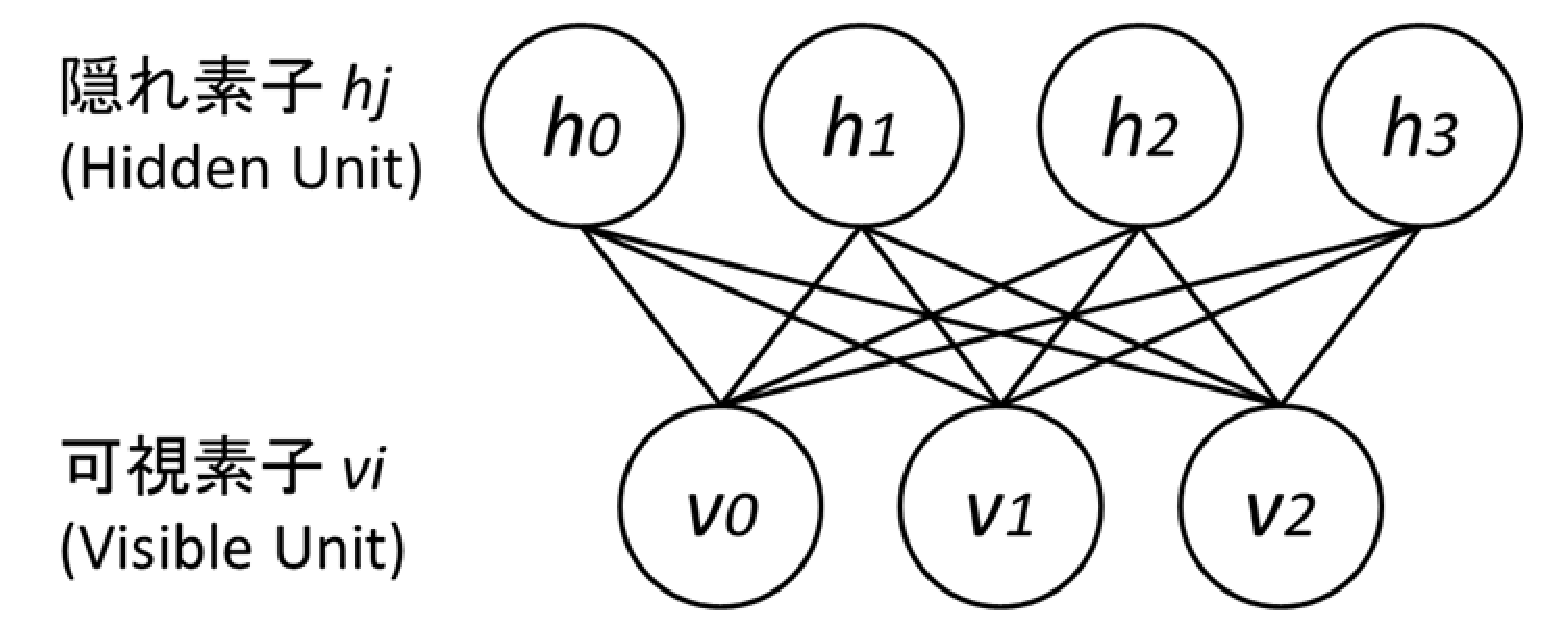
\includegraphics[scale=0.4]{./img_dl/rbm.eps}
  \caption{Restricted Boltzmann Machine}
  % \ecaption{Representations of Data} 
  \label{fig:rbm}
 \end{center}
\end{figure}

可視層と隠れ層のノードの値を示すベクトルを以下のように定義する。

\begin{eqnarray}
	\bm{v} & = & (v_0,v_1,...v_{V-1} ), \forall v_i \in {0,1} \\
	\bm{h} & = & (h_0,h_1,...h_{H-1} ), \forall h_i \in {0,1}
\end{eqnarray}

この時、RBMでは可視層と隠れ層の結合確率が以下のように定義される。

\begin{eqnarray}\label
	p(\bm{v}, \bm{h}; \theta) & = & \frac{1}{Z(\theta)}  \exp (-E(\bm{v},\bm{h};\theta)) \label{fig:rbm_p}\\
	E(\bm{v}, \bm{h}; \theta) & = & -\sum_i b_i v_i - \sum_j c_j h_j- \sum_i \sum_j v_i W_{ij} h_j \label{fig:rbm_e}
\end{eqnarray}

ここで$b_i,c_j,W_{ij}$はそれぞれ可視素子 $v_i$ のバイアス,隠れ素子 $ h_j $ のバイアス,可視素子 $ v_i $ と隠れ素子 $ h_j $ の間のウェイトパラメータである.
これらのパラメータをまとめて $ \theta $ とする.
また $ Z $ は正規化定数であり,以下のように定義される.

\begin{equation}
	Z(\theta)= \sum_{\bm{v}} \sum_{\bm{h}} \exp (-E(\bm{v}, \bm{h}; \theta))
\end{equation}

式\ref{fig:rbm_p}、式\ref{fig:rbm_e}より、片方の層の状態が入力された時、他方の層の各ノードの取る値の条件付き確率が計算できる。そのため、ある隠れ層の状態から入力を確率的に生成することが可能なため、RBMは生成モデルであるという側面を持つ。

RBMは、可視層に入力データを入れ学習させることで、隠れ層にその特徴をよく表すようなパラメータを出力することができる。この特徴を用いて、後述するDeep Belief Netのように、ディープニューラルネットワークのプレトレーニングに用いられることも多い。

\subsection{RBMの学習}\label{sec:learn}
\subsubsection{計算の概略}
RBMの学習では、可視層の観測データ$\bm{v}$に対する$p(\bm{v})$について最尤推定を行う。

$p(\bm{v})$を計算するため結合確率 $p(\bm{v},\bm{h})$ を $\bm{h}$ について周辺化する。


\begin{eqnarray}
	p(\bm{v};\theta) & = & \sum_{\bm{h}} p(\bm{v},\bm{h};\theta) \\
				& = & \sum_{\bm{h}} \frac{1}{Z(\theta)} \exp (-E(\bm{v}, \bm{h}; \theta))
\end{eqnarray}

計算の簡単のため、以下では尤度の対数をとった対数尤度を取り扱う。

\begin{eqnarray}
	J & = & < \ln p(\bm{v}; \theta) >_q \\
	  & = & < \ln \sum_{\bm{h}} p(\bm{v}, \bm{h}; \theta) >_q \\
	  & = & < \ln \sum_{\bm{h}} \exp (-E(\bm{v}, \bm{h}; \theta) >_q - \ln Z(\theta) \\
	\theta ^* & = & \argmax_\theta  J
\end{eqnarray}

ここで $<・>_q$ は確率分布 $q(\bm{v})$ の期待値を表す.

\begin{equation}
	<f(\bm{v})>_q= \sum_{\bm{v}} f(\bm{v}) q(\bm{v})
\end{equation}

また,$q(\bm{v})$ は観測データに関しての確率分布である.

\begin{equation}
	q(\bm{v}) = \frac{1}{N_{data}} \sum_n \delta(\bm{v}-\bm{v}^n)
\end{equation}

ここで$\bm{v}^k$は$k$番目の観測データを,
$ \delta(x)$は以下のように定義される関数である.

\begin{eqnarray}
\delta(x) = \begin{cases}
    1 & (n=0) \\
    0 & (otherwise)
  \end{cases}
\end{eqnarray}

ここで,対数尤度をパラメータ $ \theta $ について微分する.

\begin{eqnarray}
\frac {\partial J(\theta)}{\partial \theta} & = & 
	-<\frac{1}{\sum_{\bm{h}} \exp (-E(\bm{v}, \bm{h}; \theta))} 
	\sum_{\bm{h}} \frac{\partial E(\bm{v},\bm{h};\theta)}{\partial \theta} \exp(-E(\bm{v},\bm{h};\theta)) >_{q} \nonumber \\
	& & + \frac{1}{Z(\theta)} \sum_{\bm{v}} \sum_{\bm{h}} \frac{\partial E(\bm{v},\bm{h};\theta)}{ \partial \theta} \exp(-E(\bm{v},\bm{h};\theta))
\\
	& = & - \sum_{\bm{v}} \sum_{\bm{h}} \frac{\partial E(\bm{v},\bm{h};\theta)}{\partial \theta}
	\frac{\exp (-E(\bm{v},\bm{h};\theta)}{\sum_{\bm{h}} \exp(-E(\bm{v},\bm{h};\theta))} q(v) \nonumber \\
	& & + \frac{1}{Z(\theta)} \sum_{\bm{v}} \sum_{\bm{h}} \frac{\partial E(\bm{v},\bm{h};\theta)}{ \partial \theta} \exp(-E(\bm{v},\bm{h};\theta))
\\
	& = & < \frac{\partial E(\bm{v},\bm{h};\theta)}{ \partial \theta} >_{data}
	 - <\frac{\partial E(\bm{v},\bm{h};\theta)}{ \partial \theta} >_{model}
	 \label{eqa:pos_neg}
\end{eqnarray}

ここで、$<>_{data}$、$<>_{model}$はそれぞれ$p_{data}(\bm{v},\bm{h})=p(\bm{h}|\bm{v})q(\bm{v})$と$p_{model}(\bm{v},\bm{h})=p(\bm{v},\bm{h})$に対する期待値を表す。

ここで、第一項に関しては、可視層の状態から隠れ層の条件付き確率の厳密解が用意に計算できることから、計算はかなり容易である。一方、第二項に関しては、全ての$\bm{v}$,$\bm{h}$の組み合わせを計算しなければいけないため計算量が指数的に爆発してしまう。

したがって第二項を計算するため、 サンプリング的手法や、近似的に解を求める手法などが用いられてきた。現在では次節で説明するContrastive Divergence法と呼ばれるサンプリング手法が最も有力であり、広く用いられている。

\subsubsection{Contrastive Divergence法}
Contrastive Divergence法(CD法)は、2002年にHintonによって発表されたRBMの学習におけるサンプリング手法である。

厳密な$p(\bm{v},\bm{h})$を計算する代わりに、\bm{v}と\bm{h}をサンプリングして、$p(\bm{v},\bm{h})$を近似的に求める手法であるが、従来のギブスサンプリングとは遷移回数と可視層の初期値の選び方の点で異なる。

CD法では、\bm{v}と\bm{h}をサンプリングする際の可視層の初期値に、実際の観測データを用いる。RBMでは、各層のノードの取る値の条件付き確率は、他方の層のノードの状態にのみ依存しており、その確率はロジスティック関数 $ \sigma(x)= \frac{1}{1 + \exp(-x)} $ を用いて

\begin{eqnarray}
	p(v_i=1│\bm{h}) & = & \sigma(b_i+ \sum_j W_{ij} h_j) \\
	p(h_i=1│\bm{v}) & = & \sigma(c_i+ \sum_i v_i W_{ij}) \\
	\sigma(x)		& = & \frac{1}{1 + \exp(-x)}
\end{eqnarray}

で表されるので、入力された可視層から隠れ層の状態を求めることができる。その後、同じように求めた隠れ層の状態から可視層の状態を計算可能である。

ギブスサンプリングでは、この可視層と隠れ層の間の遷移を通常多数回行う必要があったが、CD方では少ない回数でも上手く学習が進むことが経験的に知られており、多くの場合では遷移回数が1回でも十分である。

このようにして得られた可視層の状態と条件付き確率より結合確率

\begin{eqnarray}
	p_{model}(\bm{v},\bm{h})=\frac{1}{N} \sum_k \delta( \bm{v} - \bm{v}_k ) p(\bm{h}|\bm{v}_k)
\end{eqnarray}

を求め、近似的に式\ref{eqa:pos_neg}の第二項を求める。

\section{Deep Belief Net}

ディープニューラルネットワークを教師あり学習させようとした場合、過学習や局値解に陥ってしまうと言った問題が起きることがある。
このような問題を解決するためにプレトレーニングが行われることがあるが、プレトレーニングに前述したRBMの学習を用いたものをDeep Belief Net(DBN)\cite{DBN}という.

\begin{figure}[tb]
 \begin{center}
  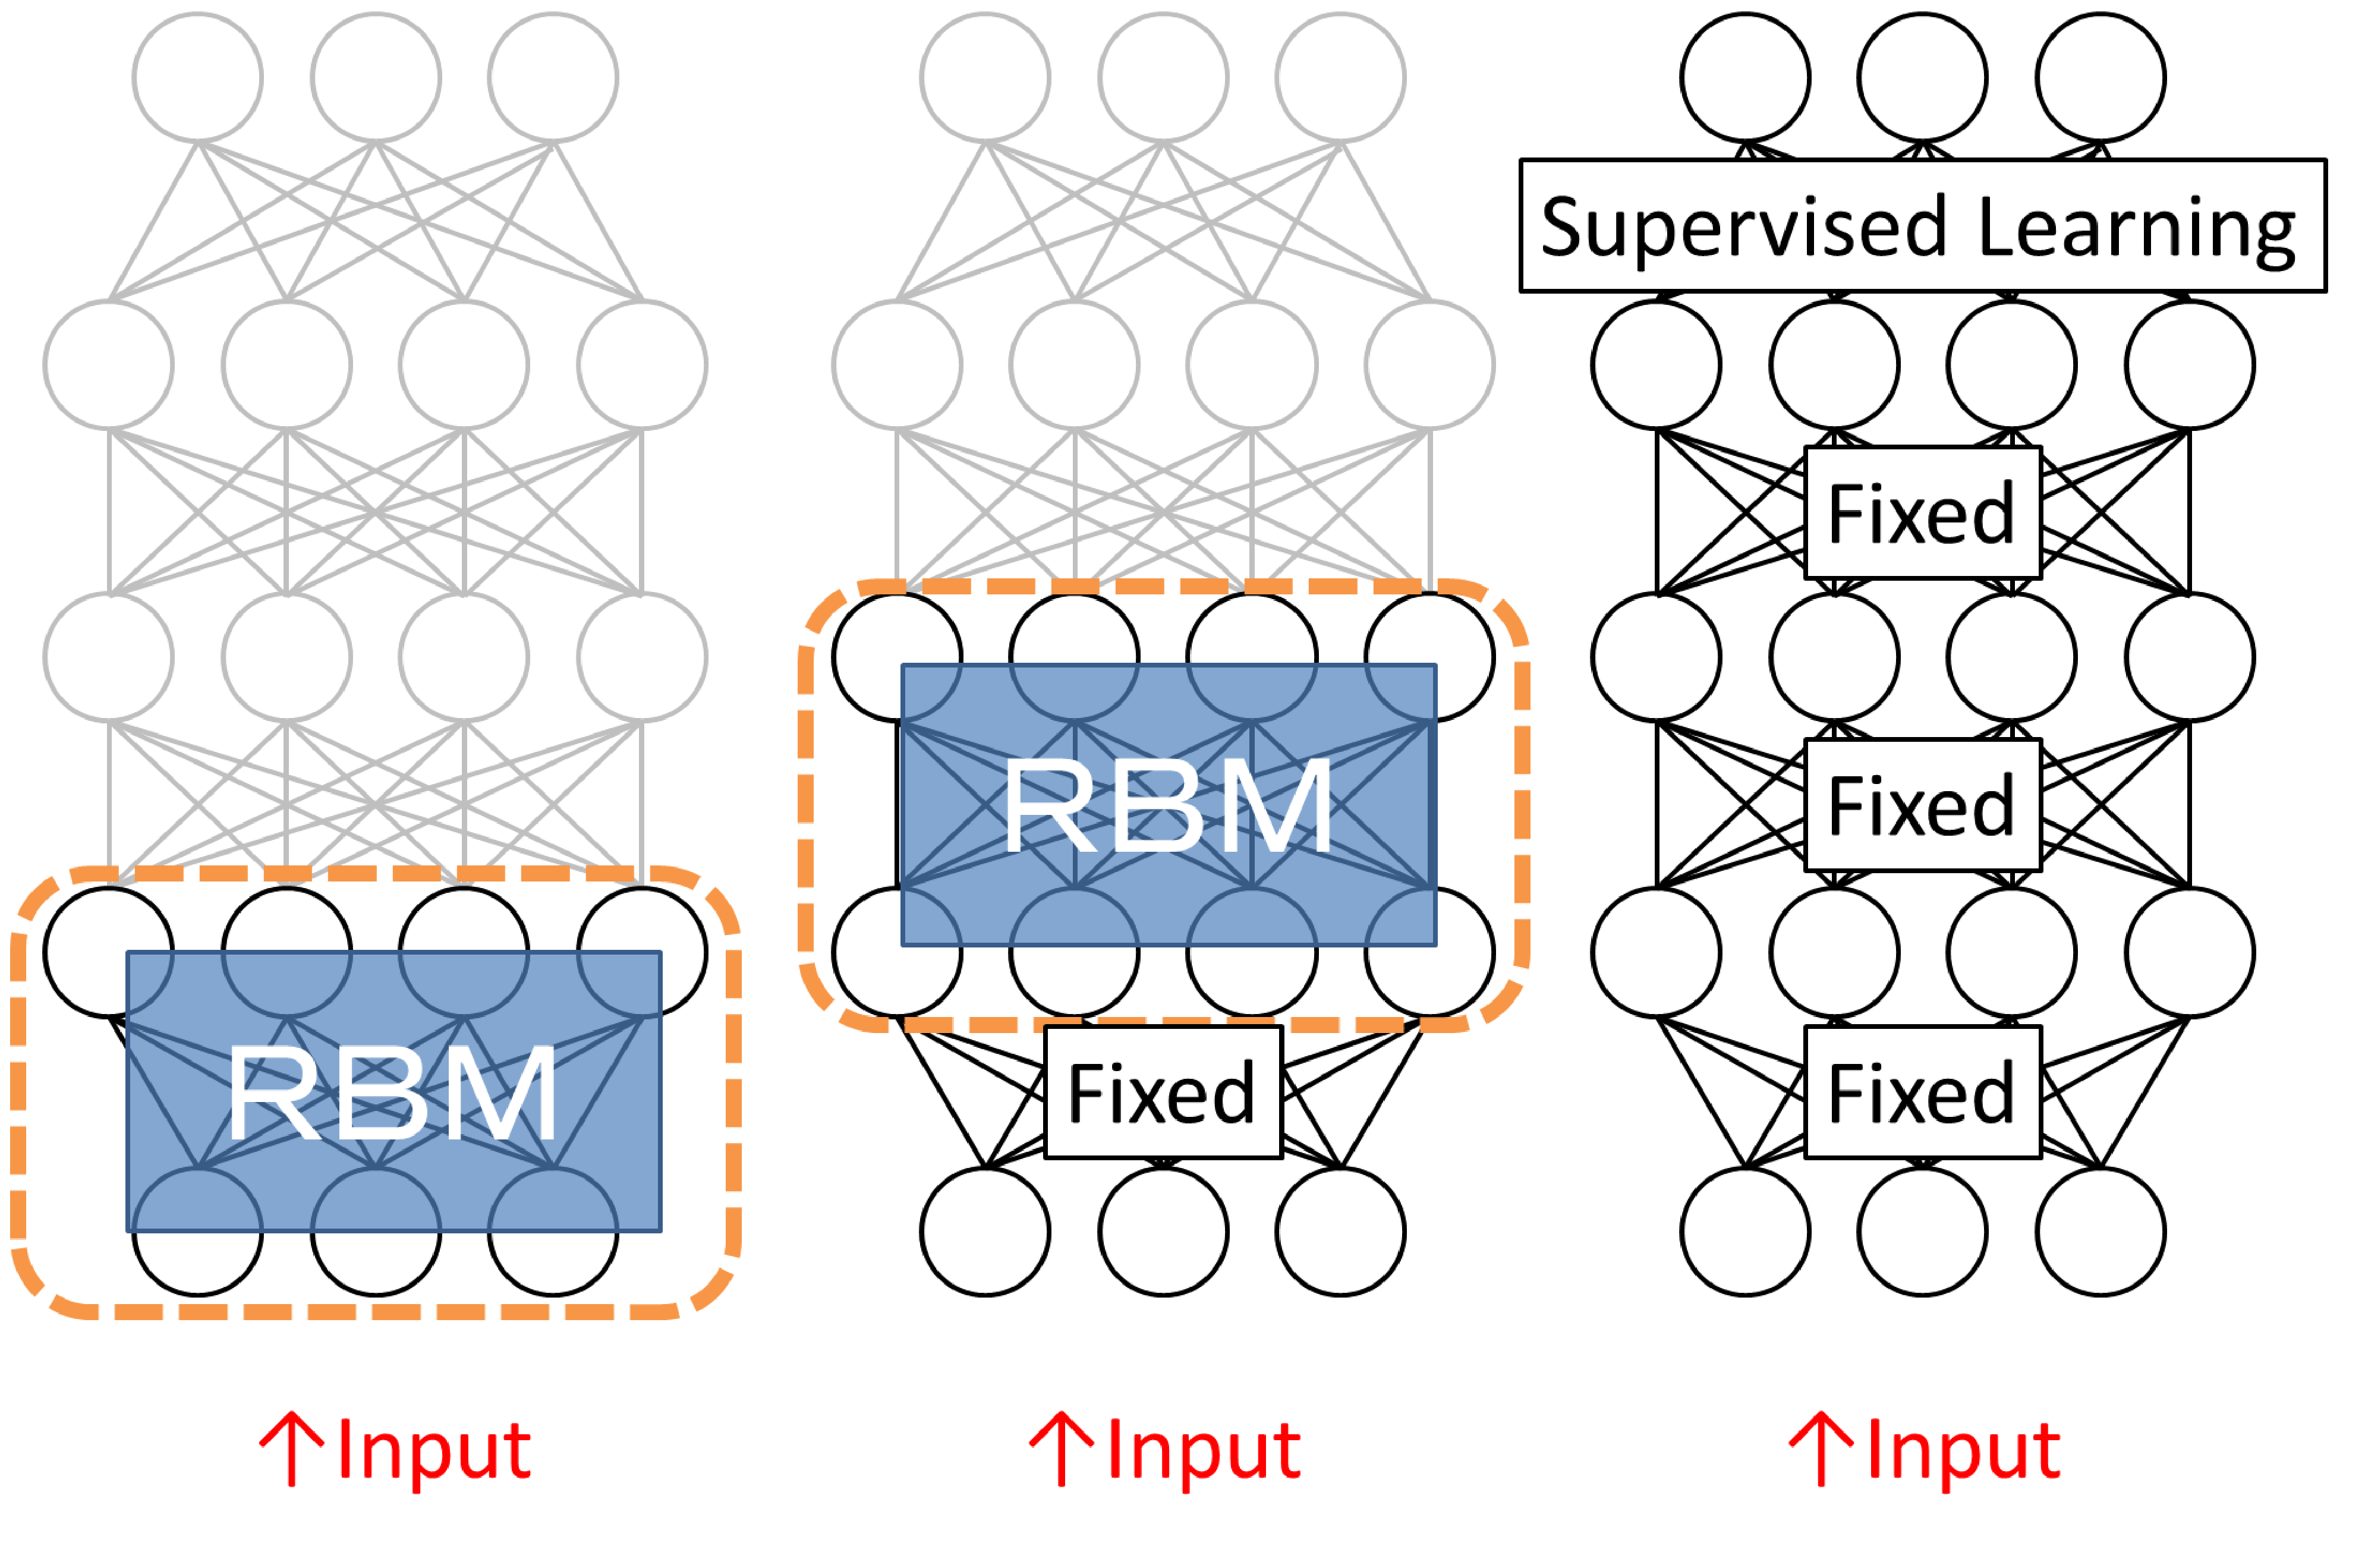
\includegraphics[scale=0.2]{./img_dl/dbn.eps}
  \hspace*{0cm}
  \vspace*{0cm} 
  \caption{DBN学習過程}
  % \ecaption{Representations of Data} でんぱ
  \label{fig:dbn}
 \end{center}
\end{figure}

図\ref{fig:dbn}にプレトレーニング\cite{glw-training}の手順を示す.

まず、ディープニューラルネットワークの第一層と第二層をRBMとみなしRBMの学習を行う。可視層に入力した入力データの特徴の表現が隠れ層に表れるというRBMの利点を、ディープニューラルネットワークのプレトレーニングに活用する。

第一層と第二層にて学習を終えた後、このRBMの重みを固定し、入力データを伝播させて表れた隠れ層の状態を新たな入力データとして、第二層と第三層を新たなRBMとみなし学習を行う。

このように連鎖的に下層から上層に向かい二層ずつRBMとみなして教師なし学習を行い、出力層では教師あり学習を行う。

このようにプレトレーニングを終えた後、ネットワーク全体で誤差逆伝播法にて教師あり学習を行う手法もしばしば用いられ、これをファインチューニングと呼ぶ。

\section{Incremental Learning-RBM(IL-RBM)}\label{sec:rbm}

提案システムのIL-RBMは追加学習を行うと既学習情報を失うというRBMの欠点を改良したものであり、追加学習を行う際に隠れ層の素子数を追加するという特徴がある。
追加する素子数を学習データセットを考慮し自動で決定するアルゴリズムと、ネットワークのエネルギーより既学習データと未学習データを判別するアルゴリズムも同時に説明する。

\subsection{隠れ層ノード数の自動決定法}\label{sec:node}
RBMの隠れ層のノード数の自動決定を行うアルゴリズム[]について説明する。文献[]において、図\ref{fig:pre_exp_line}\footnote{テキスト}に示すように、学習済みRBMのクロスエントロピーと隠れ層ノード数には以下の関係が有ることが述べられている。

\begin{itemize}
 \item  隠れ層のノード数が非常に少ない場合、ノード数にかかわらずクロスエントロピーが一定である領域が存在する場合がある。
  \item 隠れ層のノード数が不十分な場合、隠れ層のノード数を増やした際に学習済みRBMのクロスエントロピーは一般に減少し、その減少は線形に近似することができる。
  \item 隠れ層ノード数が十分な値に達した場合、隠れ層のノード数を増やしても学習済みRBMのクロスエントロピーは減少しない。  
\end{itemize}

\begin{figure}[]
\begin{center}
   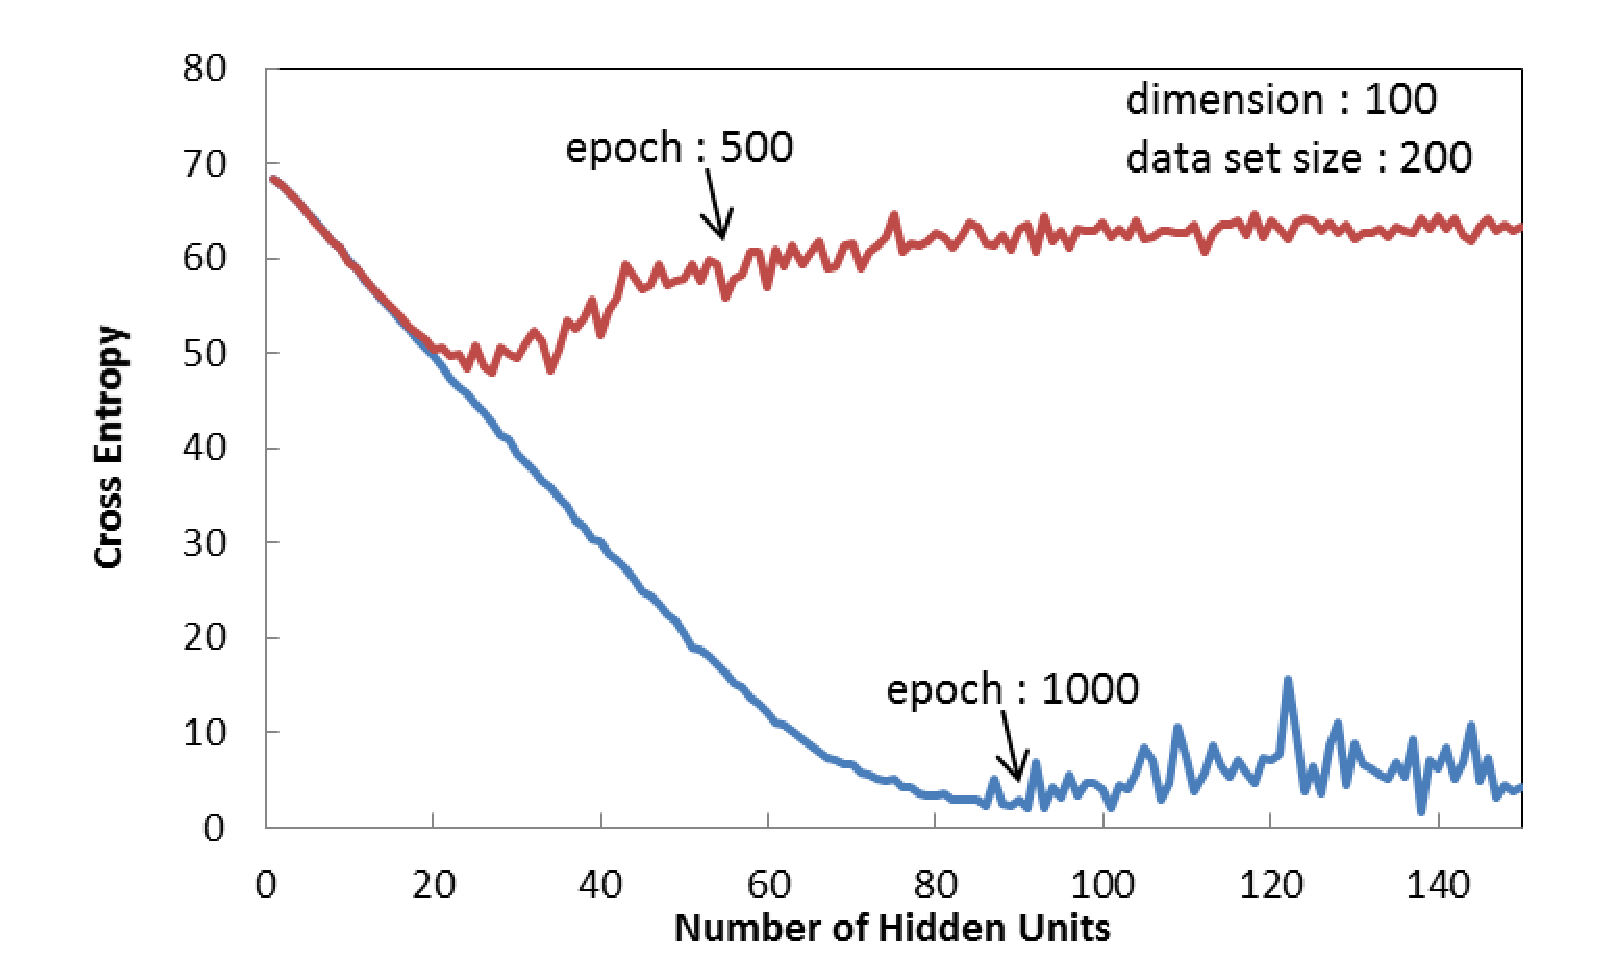
\includegraphics[scale=0.48]{./myimg/pre_exp1_c.eps} \\
   \caption{隠れ層ノード数とクロスエントロピーの関係}
  \label{fig:pre_exp_line}
\end{center}
\end{figure}

この関係を用いて、文献[]にてRBMの素子数の自動決定法が提案されている。

RBMの素子数の自動決定法は傾斜検出フェーズと傾斜予測フェーズの2つのフェーズに分けることができる。

\subsubsection{傾斜検出フェーズ}
傾斜検出フェーズは、ニューロン数にかかわらずクロスエントロピーの変化しない領域をスキップし、傾斜の始まりを正しく検出するためのフェーズである.図\ref{fig:phase1}に傾斜検出フェーズの実行過程を示す.

\begin{figure}[]
\begin{center}
  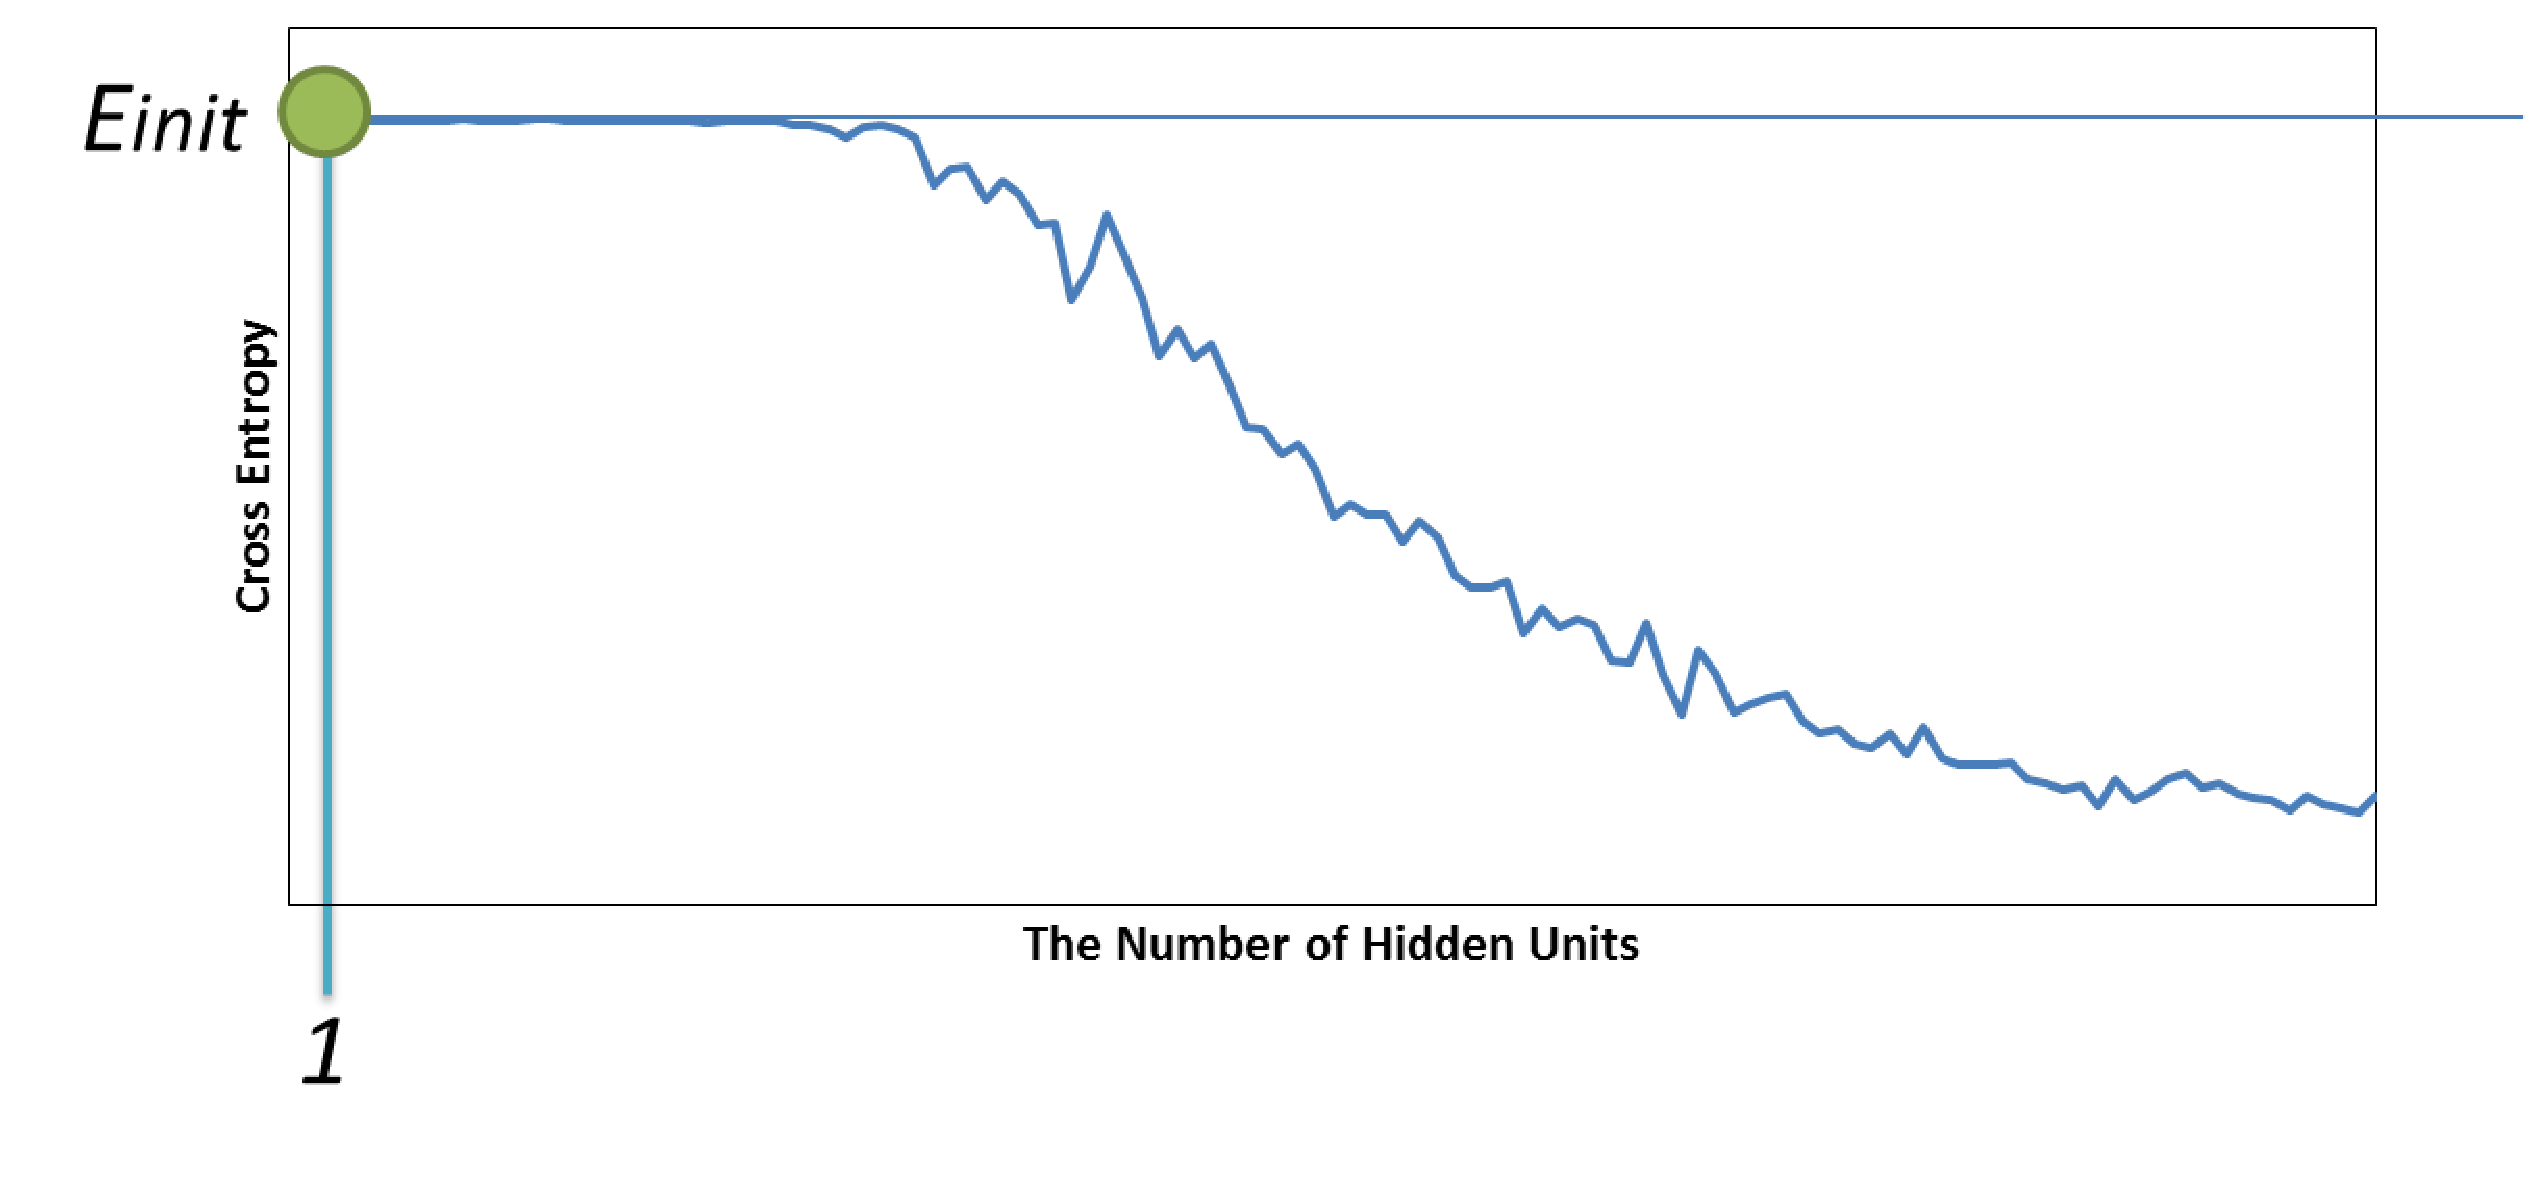
\includegraphics[scale=0.25]{./myimg/phase1_1.eps} \\
  (a) $E_{init}$の決定 \\
  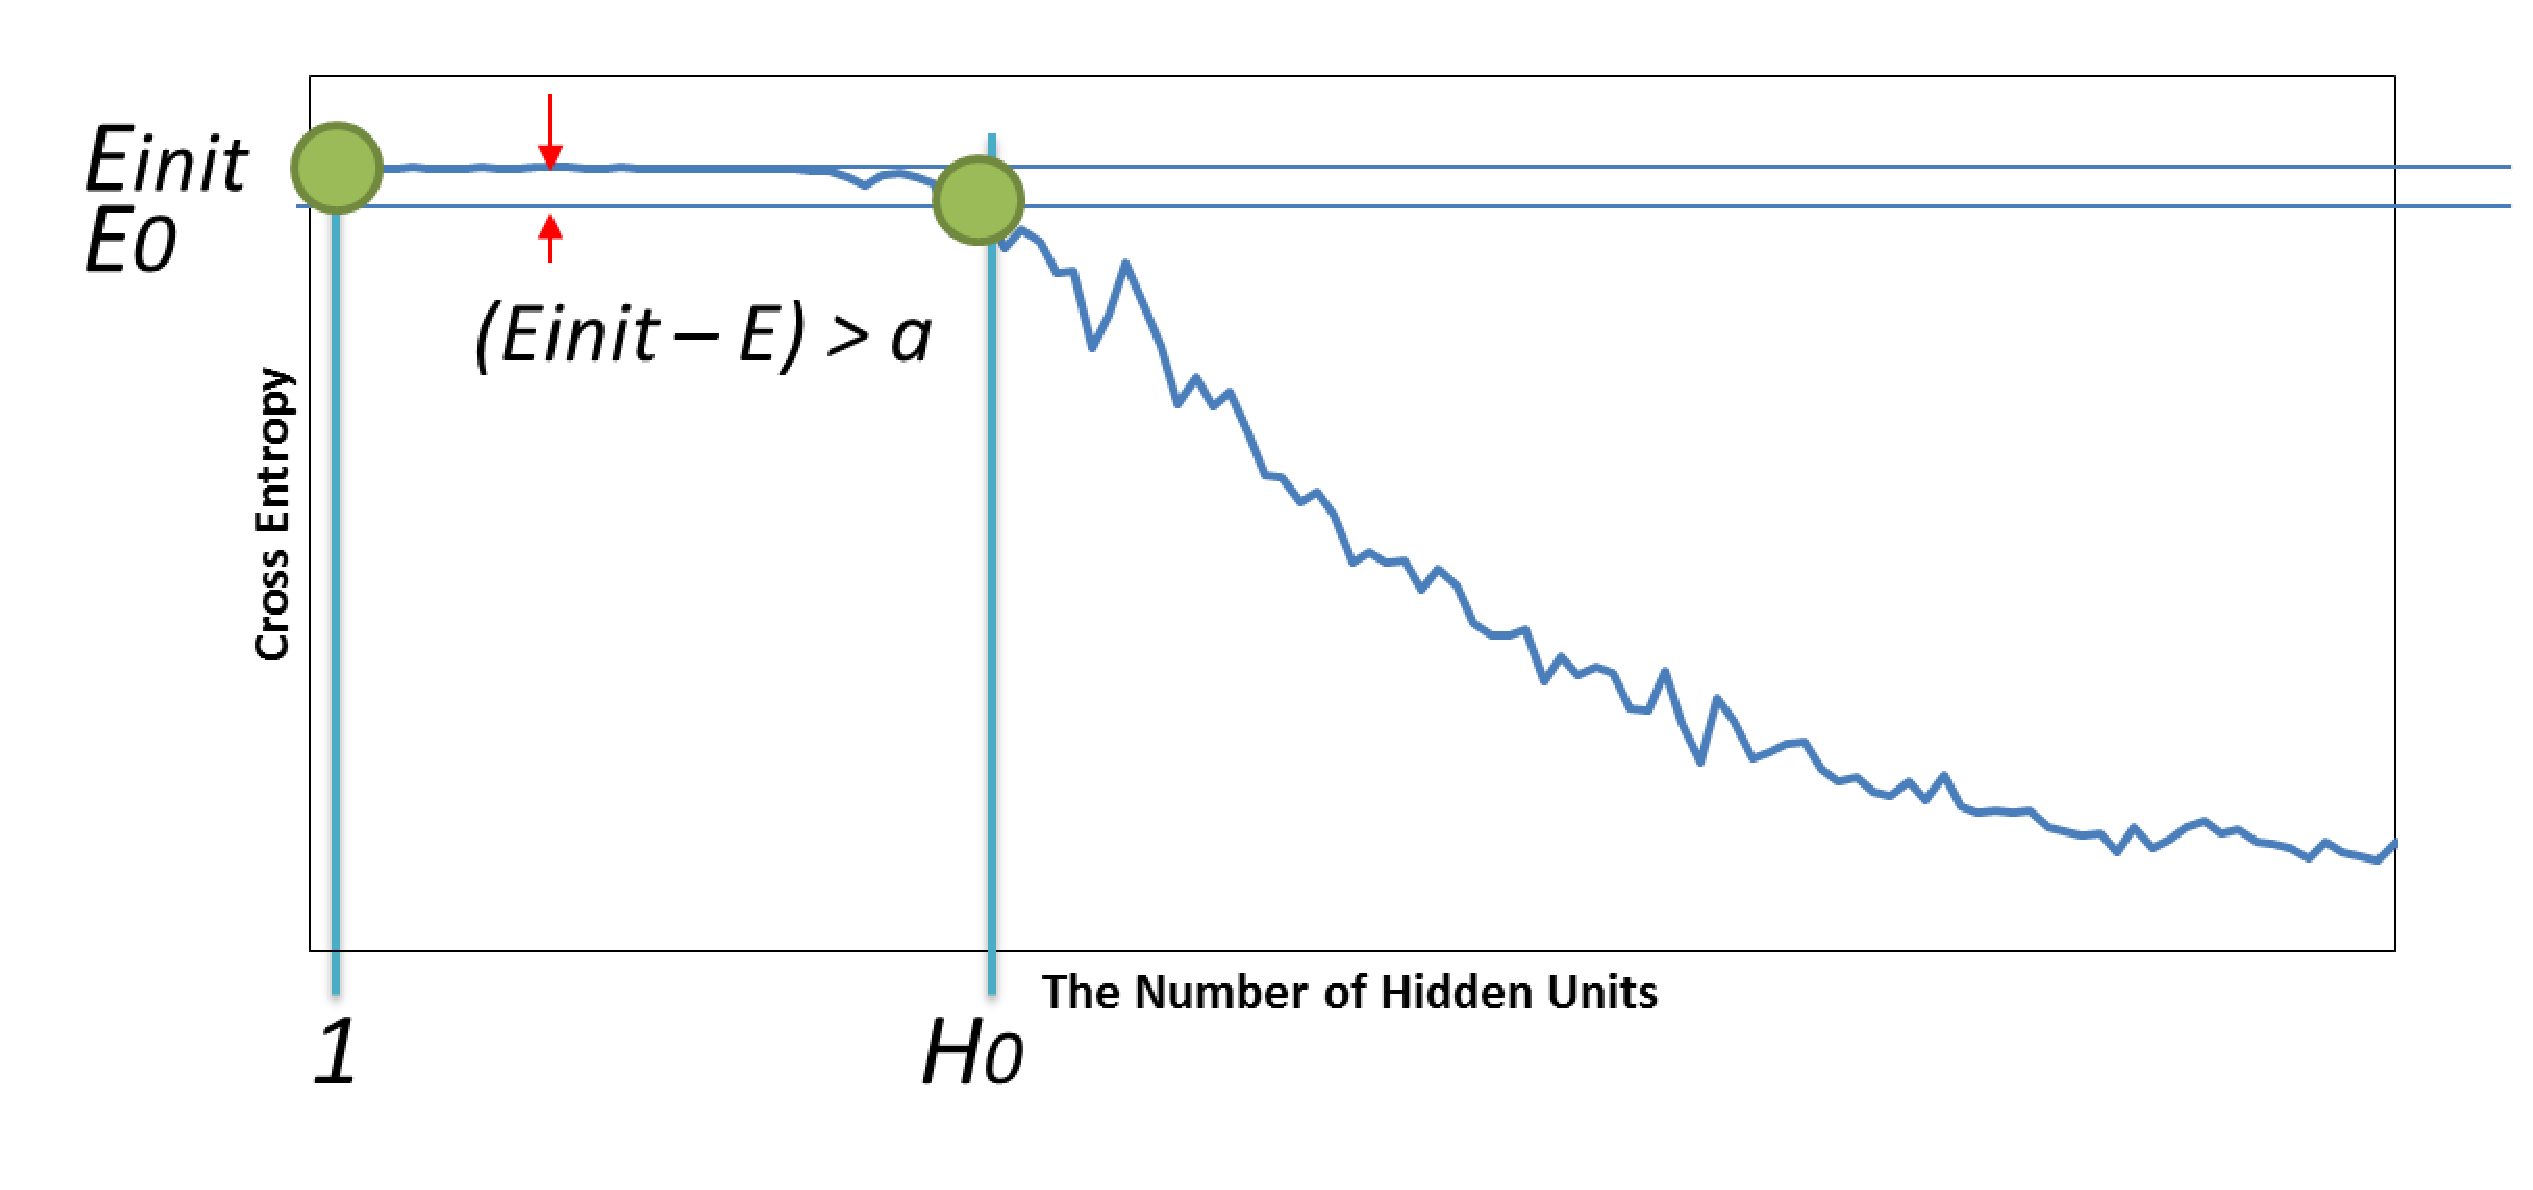
\includegraphics[scale=0.25]{./myimg/phase1_3.eps} \\
  (b) 閾値$a$との比較 \\
  \caption{傾斜検出フェーズの実行過程}
  % \ecaption{An Execution Process of Phase1}
  \label{fig:phase1}
\end{center}
\end{figure}

ニューロン数が1の時のクロスエントロピーを$E_{init}$と置く。その後、ノード数を増加させつつサンプリングしたクロスエントロピーと$E_{init}$との差がある閾値を超えた場合にクロスエントロピーの減少が始まったと判断し、その点を傾斜の開始とみなす。

傾斜の開始を検知した後、ノード数をいくつかサンプリングしてクロスエントロピーを求める。サンプリングした点から傾斜の傾きを計算し、クロスエントロピーの減少を線形で近似する。

最終的な隠れ層のノード数は、クロスエントロピーの近似式の値が0となる時のノード数が選ばれる。

\subsection{追加学習}
II-RBMでは追加学習を行う。追加学習とは、既にあるデータセットに対し学習済みのニューラルネットワークが、新たなデータセットに対し、既学習情報を失わない形で学習を行うことである。

通常のRBMの隠れ層のノード数は一定である。しかし、IL-RBMは新たなデータセットを学習する際に隠れ層のノード数を追加する操作を行う。IL-RBMの学習は次のような流れをとる。

\begin{enumerate}
  \item 初期データセットに対しIL-RBMを学習させる。
  \item 追加データセットに対し、適切な追加ノード数を決定し、Il-RBMの隠れ層にノードを追加する。
  \item 上記手順で追加したノードのみを用いて、追加データセットを学習させる。
  \item 上記2、3の手順を追加データセットの分だけ繰り返し行う。
\end{enumerate}

追加データセットに対する適切な追加ノード数の決定には\ref{sec:node}節で説明したノード数の自動決定法を用いる。


%%%%%%%%%%%%%%%%%
%%%%%
%%%%%
%%%%%%%%%
%%%%%%%
%%%%
%%%%%%%%%%%

\subsection{システム全体の流れ}



本システムは、強化学習の基本的な考え方に則り、"環境"と"エージェント"が”行動"と"報酬"により相互に影響を及ぼし合うように構成されている。

システムの流れは以下のとおりである。

\begin{enumerate}
  \item 二つのエージェントを定義する。
  \item 先行のエージェントに盤面の状態を与える。
  \item 先行のエージェントは盤面の状態から行動を選択する。
  \item 環境は、エージェントの行動を受け取り、自身の状態を更新する。
  \item 環境の状態に応じて、エージェントに報酬を与える。
  \item 環境の状態が終了条件を満たせばゲームを終了する。
  \item 上記手順を先攻、後攻を交代し繰り返す。
\end{enumerate}



環境部分は、常にある状態をを持ち、その状態はエージェントの行動によって変化させられる。また、環境部はその状態とエージェントの行動によってエージェントに与える報酬を決定する。

\section{Incremental Learning-RBM(IL-RBM)}

この節では、本システムの根幹となるIL-RBMについて説明する。
IL-RBMは追加学習を行うと既学習情報を失うというRBMの欠点を改良したものである。

\subsection{追加学習}
IL-RBMでは追加学習を行う。追加学習とは、既にあるデータセットに対し学習済みのニューラルネットワークが、新たなデータセットに対し、既学習情報を失わない形で学習を行うことである。

通常のRBMの隠れ層のノード数は一定である。しかし、IL-RBMは新たなデータセットを学習する際に隠れ層のノード数を追加する操作を行う。IL-RBMの学習は次のような流れをとる。

\begin{enumerate}
  \item 初期データセットに対しIL-RBMを学習させる。
  \item 追加データセットに対し、適切な追加ノード数を決定し、Il-RBMの隠れ層にノードを追加する。
  \item 上記手順で追加したノードのみを用いて、追加データセットを学習させる。
  \item 上記2、3の手順を追加データセットの分だけ繰り返し行う。
\end{enumerate}





\subsection{未学習データセットの判別}
エージェントに与えられたあるデータを既学習であるか、未学習であるかを判別する手法について述べる。
エージェントに与えられたデータの既学習判定にRBMのエネルギーを用いる。RBMは学習済みのデータに対して、エネルギーが低くなる、という特徴を持つため、データを入力した際のRBMのエネルギーを見ることで入力されたデータが既学習であるか、未学習であるかを判別することができる。






%!TEX root = ../main.tex
\chapter{IL-RBMの強化学習への応用}
この章は\ref{sec:ilrbm}にて説明したIL-RBMの,本システムにおける強化学習への応用について説明する。


\subsection{強化学習}
強化学習とは、あるエージェントがある環境内にて、得られる報酬を最大化するような行動を学習するような機械学習のことである。

強化学習には重要な4つの概念がある。

\begin{itemize}
  \item 環境 … エージェントの行動に応じて、報酬をエージェントに与える。また、エージェントの行動に応じて、エージェントの観測する環境も更新される。
  \item 報酬 … エージェントの行動に応じて環境からエージェントに与えられる。この得られる報酬を最大化するようエージェントは行動を学習する。
  \item 行動  … エージェントは観測した環境に応じて、行動を選択する。
  \item エージェント … 環境を観測し、報酬を受け取り、行動を選択する。
\end{itemize}

明確な教師データが与えられる教師あり学習や、全く教師データが与えられない教師なし学習と異なり、報酬という限定されたフィードバックのみが与えられる点に特徴がある。
不確実な環境を取り扱えるという点で、応用上非常に有望な機械学習手法の一つである。

\subsection{エージェントの概要}
エージェントの概要について具体的に説明する。

本システムで用いたエージェントは、IL-RBMと出力層からなるDBN(以下、IL-DBN)を用いている。このIL-DBNは入力データを環境、出力を行動として学習する。
エージェントは、常に今自分が置かれている環境を観測することが可能であり、環境から報酬を与えられた場合には、それを感知することが可能である。

エージェントは環境と行動の組からなるデータセットを自動的に構築し、そのデータセットを逐次的に学習することで、最適行動を学習する。
また、IL-RBMのエネルギーに注目することで、未学習データセットを検出できるという特徴を用い、後述するサブゴールを獲得し、長期的な戦略を獲得することが可能である。

\subsection{未学習データ判定法}

\ref{sec:learn}で説明したとおり、RBMは以下に$J$で表される対数尤度を最大化するように学習が行われる。すなわち、エネルギー$E$を最小化するように学習が行われることと同値である。

\begin{eqnarray}
	p(\bm{v}, \bm{h}; \theta) & = & \frac{1}{Z(\theta)}  \exp (-E(\bm{v},\bm{h};\theta)) \nonumber \\
	E(\bm{v}, \bm{h}; \theta) & = & -\sum_i b_i v_i - \sum_j c_j h_j- \sum_i \sum_j v_i W_{ij} h_j \nonumber \\
	p(\bm{v};\theta) & = & \sum_{\bm{h}} p(\bm{v},\bm{h};\theta) \nonumber \\
			& = & \sum_{\bm{h}} \frac{1}{Z(\theta)} \exp (-E(\bm{v}, \bm{h}; \theta)) \nonumber \\
	J & = & < \ln \sum_{\bm{h}} p(\bm{v}, \bm{h}; \theta) >_q \nonumber \\
	  & = & < \ln \sum_{\bm{h}} \exp (-E(\bm{v}, \bm{h}; \theta) >_q - \ln Z(\theta) \nonumber 
\end{eqnarray}

したがって、学習済みRBMは既学習データが入力された場合はエネルギーが低くなり、未学習データが入力された場合にはエネルギーが高くなる。この原理を応用し、あるデータが入力された際のRBMのエネルギーを判定することで未学習データか既学習データかの判定を行う。

未学習データを入力した際のエネルギーと既学習データを入力した際のエネルギーをそれぞれ記録しておき、この値に基づいてある閾値を決定し、未学習か既学習か不明であるデータが入力された際のRBMのエネルギーが、この閾値を上回れば未学習、下回れば既学習と判定する。

\subsection{データセットの獲得}

本システムがデータセットを環境中から自動で学習するメカニズムについて説明する。
以下、三目並べタスクの最適行動を学習するエージェントを例に説明する。

学習エージェントが対戦相手と三目並べを行う環境下で、三目並べに勝利した場合と敗北した場合にそれぞれ正の報酬と負の報酬を与えられるとする。この時、エージェントが観測する環境は盤面の状態であり、出力する行動は次に選択する手の盤面上の位置となる。

\subsubsection{勝利データセットの獲得}
まず、エージェントは勝利データセットを収集する。ある行動を出力した際、盤面が勝利条件を満たし、正の報酬が与えられたとする。その勝利条件を満たした際の行動と、その行動をとった際の環境を組みにしてデータセットとしてエージェントは保存する。

データセットがある一定数に達した場合、または試行回数が一定数に達した場合、エージェントは保存したデータセットを用いて学習を行う。

\subsubsection{サブゴールの獲得}
前述した、既学習、未学習判定を用いてサブゴールを獲得し、長期的な戦略を獲得するメカニズムについて説明する。

勝利データセットの獲得において、盤面が勝利条件を満たした場合、その時にとった行動と、行動を選択した際の環境を組みにしてデータセットとして保存した。
この場合、勝利条件を満たした盤面の状態をゴールとしてデータセットを採集している。

サブゴールとは、ゴールにつながり得る環境の状態を指す。
サブゴールを適切に設定し、サブゴールに至る行動と、その行動を選択した際の環境を更にデータセットに加える事で、長期的な戦略を獲得することができる。

サブゴールの設定方法について説明する。ある行動を選択し、環境が更新されたとする。
その際の環境をエージェントのRBMが既学習であるか未学習であるかを前述したエネルギーによる判定法で判定する。
そして、得られた環境が既学習であった場合、その環境はゴールへと至る可能性が高いため、その環境をサブゴールとして設定する。
そして、サブゴールに至る直前の環境と、その状態にて選択した行動をデータセットとして新たに保存し、追加学習を行う。

このようにして、サブゴールについても学習したIL-RBMは、また新たに"サブゴールのサブゴール"を扱うことが可能になる。観測された環境が、既に学習済みであるサブゴールである環境と一致、近似すると判定された場合、さらにその環境に至る行動とその直前の環境をデータセットとして加えることで、サブゴールのサブゴールを学習でき、長期的な戦略を獲得することが可能である。

\subsection{負のネットワーク、負のサブゴール}
前述したサブゴールの設定法には負の報酬と行動の抑制を扱えない、という欠点があった。
あるRBMがある環境を表す入力データを未学習か既学習か判定できたとしても、その環境が正の報酬に紐付いているか、負の報酬に紐付いているかを判定できないからである。

そこで、負の報酬と負の報酬を得る環境へ至る行動を抑制するために負の報酬をあつかうネットワークをエージェントに追加することにした。

エージェントはIL-RBMを二つ使用する。それぞれ正の報酬を扱うネットワークと負の報酬を扱うネットワークである。
また、保持するデータセットも二種類用意する。正の報酬を得ることのできるゴールに至る行動と、その直前の環境の組、サブゴールに至る行動とその直前の環境の組をデータセットとして扱う正のデータセットと、負の報酬について同様に扱う負のデータセットである。

負のデータセットを扱う負のネットワークでは、負の報酬を得ることになるゴール、サブゴールに至る行動が出力され、その直前の環境が入力データとなる。したがって、観測された環境をこのネットワークに入力した際の出力された行動は抑制されるべき行動である。

本エージェントでは負のネットワークからの出力を正のネットワークからの出力から引くことで、負の報酬を得る環境へ至る行動を抑制している。しかし、正のネットワークと負のネットワークを同列に扱うべきか、荷重をかけどちらかを優先すべきかなどは研究途中である。


%%!TEX root = ../main.tex
\chapter{評価実験}
本研究では、提案手法の強化学習への妥当性の検証のため、三目並べタスクを行った。実験を行うために制作したシステムの詳細について述べた後、実験と結果についての報告と考察を行う。

\section{三目並べタスクの強化学習システムの詳細}
本システムは強化学習の基本的な考え方に則り、環境とエージェントの相互作用を取り扱う。

\subsection{環境部}
環境部はエージェントと環境の相互作用を制御するmainオブジェクトと、三目並べタスクの詳細の動作、情報を制御するThreePieceオブジェクトからなる。

\subsection{mainオブジェクト}
mainオブジェクトは、プログラム全体の制御を行う。

まず、行うタスクを定義する。今回行うタスクは三目並べであるためThreePieceオブジェクトをタスクとして定義する。その後、タスクの要請する数のエージェントを定義する。今回の実験では、先行のエージェントをランダムエージェント、後攻のエージェントをIL-DBNエージェントとした。

その他、エージェントと環境の相互作用を制御し、三目並べの終了時にThreePieceオブジェクトとエージェントのリセットを行ったり、三目並べを何ターン行うかの制御、それぞれのエージェント数の勝利数の保持を行う。

\subsection{ThreePieceオブジェクト}
ThreePieceオブジェクトは三目並べタスクを実際に執り行う。
ThreePieceオブジェクトはターン制でそれぞれのエージェントに盤面の情報を渡し、行動情報を受け取る。
盤面の情報の次元数や行動情報の形式はThreePieceオブジェクトが決定し、エージェントがアーキテクチャをその形式に合わせる。

盤面の情報はそれぞれのマスに対し、空白ならば(0,0),白石が置かれていれば(0,1)、黒石が置かれていれば(1,0)の2bitで表現する。したがって9マス全体の表現は18次元の(0,0,0,1,1,0,0,0,0,1,0,0,0,0,0,0,1,0)のような表現になる。

一方エージェントの行動は0〜8の整数値で表される。それぞれの数値が石を置く盤面上の位置を示している。

%一方、エージェントの行動は9次元のベクトルで表現される。配置する石の位置に対応する次元の値のみ1で、それ以外は0のベクトルで表す。

ThreePieceオブジェクトはエージェントから渡された石の置き位置を示す値がルール上正当なものかを判定する。エージェントが石を置こうとしている場所に既に石が置かれている場合はエージェントに再度行動を選択するように命令する。指定された石の置き位置が正当であれば、オブジェクトの保持する盤面の状態を更新する。

その後、盤面の状態が三目並べの終了条件を満たしているかを判定する。盤面の状態を監視し、縦、横、斜めいずれかの方向に石が3つ並んでいれば、勝利エージェントへ報酬1を、敗北エージェントへ報酬-1を与える。

\subsection{エージェント部}
エージェントは基本的なエージェントの振る舞いを規定するAgentクラスがあり、それを継承することでそれぞれのAgentのクラスが作られている。

エージェントは環境から盤面状態を受け取った後、行動選択を行う。ランダムエージェントであれば0〜8で乱数を返し、学習エージェントは学習した行動を出力する。

環境が行動を受け取った後、エージェントは環境から報酬を受け取る。学習エージェントは報酬に応じて学習を行う。その学習の具体的なプロセスについては後述する。

\susubbsection{学習エージェント}
学習エージェントは次のような流れで学習を行う。



\begin{enumerate}
  \item データセットを構築する。
  \item
  \item 先行のエージェントは盤面の状態から行動を選択する。
  \item 環境は、エージェントの行動を受け取り、自身の状態を更新する。
  \item 環境の状態に応じて、エージェントに報酬を与える。
  \item 環境の状態が終了条件を満たせばゲームを終了する。
  \item 上記手順を先攻、後攻を交代し繰り返す。
\end{enumerate}


\section{予備実験と各種パラメータの決定}

\section{提案手法の評価実験}

\begin{itemize}
\item [(1)]対話システムの性能として
\item [(2)]ユーモアの質として
\end{itemize}
表\ref{ht:Grice}に(1)の評価項目,\ref{ht:Humor}に(2)の評価項目を示す。
\chapter{結論}
%本論文ではユーザの発話を考慮したユーモアを有する非タスク指向型対話システムを提案した。\\
%\hspace{1zw}提案システムは,ユーザにテキスト入力で対話を行ってもらった。その文から感情や極性,文体を読み取り,予備実験の基,適切なタイミングでかつ,適切な内容でユーモアを発話するようにした。そうすることで,ユーモアの効果を最大限に引き出すようにした。\\
%\hspace{1zw}評価実験の結果から,非タスク指向型対話システムにおけるユーモアの重要性を示し,そのユーモアのタイミングと内容の考慮の有効性を示した。\\
%\hspace{1zw}今後は,ユーザに音声入力を行ってもらい,イントネーションや間などユーザから得る情報を増やす。それらの情報も同時に利用することで,より適切なユーモアのタイミングと内容を推定するようにする。


本論文ではユーザの発話を考慮したユーモアを有する非タスク指向型対話システムを提案した。\\
\hspace{1zw}提案システムでは,ユーザの発話文から,ユーザの感情や極性,またその文体を推定し,それらの基,ユーモアを用いるか否かを決定した。
またユーモアを用いる際は,予めユーモアの内容を,提唱されたユーモアの種類に応じ,細分化されたユーモアの中から決定した。\\
\hspace{1zw}その結果,評価実験から対話システムの性能とユーモアの質の向上が見られた。\\
\hspace{1zw}今後は,入力文の中に,ユーモア生成に必要な情報が無くても,ユーモアの性質を活かしたテンプレートではなく,動的なユーモアを応答するよう心がけたい。
そのためには,ユーザとの会話でユーザに関する情報,つまり知識を獲得し,そのユーザに応じたユーモアの応答を行うようにし,ユーモアの質を上げる。\\
\hspace{1zw}また,発話をテキスト入力ではなく,音声入力に転換し,イントネーションや間などユーザから得る情報を増やす。その情報も利用することで,より適切なユーモアを応答するようにして,システムの向上化を目指す。
%\謝辞
本研究を行うに当たって,丁寧な御指導をして頂いた萩原将文教授には深く感謝を致します。\\
\hspace{1zw}システムを構築する際のユーモアを含む応答文作成に関して,吉田裕介様が作成して頂いた言語資源やプログラムには大変お世話になりました。改めて感謝致します。\\
\hspace{1zw}また,システムを構築する際に,様々な言語資源を提供して下さった作成者及び関係者の方々に厚く御礼を申し上げます。\\
\hspace{1zw}さらに,予備実験と評価実験に協力して頂いた研究室の皆様,ならび友人の方々に感謝を意を示します。\\
\hspace{1zw}最後に,私を経済的,精神的に支えて下さった両親には言葉にはできないものがあります。この謝辞をもってそれを示したく思います。

%\bibliographystyle{jecon.bst}
\bibliography{./reference/reference}

\appendix

%\chapter{評価実験の対話データ}
ここでは、評価実験の際に実際に行われた対話を本編で記した以外のものを記す。

\begin{longtable}{| c | p{15zw} | p{15zw}|}
\caption{20代女性の対話例}
%\label{fig:samplenoboke}
\endhead
%\begin{tabular*}{70mm}{@{\extracolsep{\fill}}|c|c|}\hline %ココ
\hline
{\em 話者} & {\em 発話文} & {\em 応答パターン}\\
\hline
\hline
usr & こんにちは & \\
sys & こんにちは & テンプレート応答\\
usr & 調子はどうですか? & \\
sys & 怒りたい & 攻撃ユーモア(テンプレート応答)\\
usr & どうしてですか? & \\
sys & 他の話をしようぜよ & 応答生成不可or応答候補無し\\
usr & 天気がいいですね & \\
sys & それはいいね! & 極性を考慮した相槌\\
usr & 散歩したいです & \\
sys & え?ランコしたいです?私の聞き間違いですか?? & 遊戯ユーモア(ダジャレ)\\
usr & 聞き間違いです & \\
sys & それは辛いね & 極性を考慮した相槌\\
usr & 辛いです & \\
sys & 君を励ましたかった & 支援ユーモア(テンプレート応答)\\
usr & ありがとう & \\
sys & どういたしまして & テンプレート\\
usr & 元気ですか & \\
sys & さすがです & 相槌\\
\hline
\end{longtable}


\begin{longtable}{| c | p{15zw} | p{15zw}|}
\caption{20代男性の対話例}
%\label{fig:samplenoboke}
\endhead
%\begin{tabular*}{70mm}{@{\extracolsep{\fill}}|c|c|}\hline %ココ
\hline
{\em 話者} & {\em 発話文} & {\em 応答パターン}\\
\hline
\hline
usr & こんにちは & \\
sys & こんにちは & テンプレート応答\\
usr & よろしくおねがいします & \\
sys & うるさいですね & 攻撃ユーモア(テンプレート応答) \\
usr & ごめんなさい & \\
sys & いいえ & テンプレート\\
usr & 最近寒いですね & \\
sys & 他の話をしないか? & 応答生成不可or応答候補無し\\
usr & お金が欲しい & \\
sys & なんて? & 攻撃ユーモア(テンプレート応答)\\
usr & 卒論つらい & \\
sys & なるほどねー。 & 相槌\\
usr & 死にたい & \\
sys & あなたは子孫繁栄が死ねばよかったのに。 & 攻撃ユーモア(ツッコミ)\\
usr & お腹が好きました & \\
sys & 私も好きです & テンプレート応答\\
usr & 僕は嫌いです & \\
sys & なんて?ダツは嫌いです?私の聞き間違いですか?? & 遊戯ユーモア(ダジャレ)\\
usr & あなたの聞き間違いです & \\
sys & あなたを悲しませたい & 攻撃ユーモア(テンプレート応答)\\
usr & やめてください & \\
sys & 他の話をしようぜ? & 応答生成不可or応答候補無し\\
usr & いいよ & \\
sys & 他の話をしようぜ? & 応答生成不可or応答候補無し\\
usr & 音楽が好きです & \\
sys & 私も好きです & テンプレート応答\\
usr & 福神漬が嫌いです & \\
sys & あなたを楽しませたい & 遊戯ユーモア(テンプレート応答)\\
usr & もっと頑張って & \\
sys & 怒りたい & 攻撃ユーモア(テンプレート応答)\\
usr & やめて & \\
sys & え、そうなんだ & 相槌\\
usr & 怒られるのは嫌いだよ & \\
sys & なんて?怒られるのはキレイだよ?私の聞き間違いですか?? & \\
usr & あなたの名前は? & \\
sys & ゼロです。以後お見知りおきを & テンプレート応答\\
usr & よろしくお願いします & \\
sys & こちらこそよろしくお願いします & テンプレート応答\\
usr & かっこいい名前ですね & \\
sys & なんて?かっこいいナナイですね?私の聞き間違いですか?? & \\
usr & かわいい女の子が好き & \\
sys & 私も好きです & テンプレート応答\\
usr & かわいい男の子も好き & \\
sys & 私も好きです & テンプレート応答\\
usr & へえ & \\
sys & 他の話をしようぜ? & 応答生成不可or応答候補無し\\
usr & いいよ & \\
sys & あなたを悲しませたい & 攻撃ユーモア(テンプレート応答)\\
usr & もうやめようよ & \\
sys & 他の話をしようぜよ & 応答生成不可or応答候補無し\\
usr & やめよう & \\
sys & 他の話をしようぜ? & 応答生成不可or応答候補無し\\
usr & 嫌です & \\
sys & あなたを楽しませたい & 遊戯ユーモア(テンプレート応答)\\
usr & 嬉しい & \\
sys & あなたを悲しませたい & 攻撃ユーモア(テンプレート応答)\\
usr & お前きらい & \\
sys & 今から1年経てば、その辛さもどうでも良くなってるよ & \\
usr & いいこと言うね & \\
sys & ごめん、応答が思いつかない & 応答生成不可or応答候補無し\\
usr & もうやめようか & \\
sys & 他の話をしようぜ? & 応答生成不可or応答候補無し\\
usr & ばいばい & \\
sys & へー、ほんとにぃ & 相槌\\
\hline
\end{longtable}



%\chapter{予備実験で得た結果}
ここでは、予備実験で得たユーモアのタイミングや内容を考慮する材料となった表の例を示す。\\
\hspace{1zw}例1はある男性の結果,例2はある女性の結果である。

\begin{table}
\begin{center}
\caption{極性の例1}
\label{tb:ex1PN}
\begin{tabular}{|c|c|c|p{6em}|p{6em}|p{6em}|}
\hline
\multicolumn{1}{|c}{} & \multicolumn{1}{c}{} & \multicolumn{1}{c|}{} & \multicolumn{3}{c|}{全体的にどの極性が多いか} \\
\cline{4-6}
\multicolumn{1}{|c}{} & \multicolumn{1}{c}{} & \multicolumn{1}{c|}{} & \multicolumn{1}{c|}P & \multicolumn{1}{c|}N & \multicolumn{1}{c|}E \\
\hline
 &  & 攻撃ユーモア & \hspace{2.4zw}0.6 & \hspace{2.4zw}0.2 & \hspace{2.4zw}0.2 \\\cline{3-6}
 & P & 支援ユーモア & \hspace{2.4zw}0.3 & \hspace{2.4zw}0.6 & \hspace{2.4zw}0.5 \\\cline{3-6}
 &  & 遊戯ユーモア & \hspace{2.4zw}0.8 & \hspace{2.4zw}0.4 & \hspace{2.4zw}0.3 \\\cline{3-6}
 &  & ユーモア無し & \hspace{2.4zw}0.2 & \hspace{2.4zw}0.2 & \hspace{2.4zw}0.0 \\\cline{2-6}
 &  & 攻撃ユーモア & \hspace{2.4zw}0.6 & \hspace{2.4zw}0.7 & \hspace{2.4zw}0.0 \\\cline{3-6}
1つ前の & N & 支援ユーモア & \hspace{2.4zw}0.7 & \hspace{2.4zw}0.7 & \hspace{2.4zw}0.5 \\\cline{3-6}
ユーザの &  & 遊戯ユーモア & \hspace{2.4zw}0.5 & \hspace{2.4zw}0.5 & \hspace{2.4zw}0.5 \\\cline{3-6}
発話極性 &  & ユーモア無し & \hspace{2.4zw}0.2 & \hspace{2.4zw}0.2 & \hspace{2.4zw}0.0 \\\cline{2-6}
 &  & 攻撃ユーモア & \hspace{2.4zw}0.6 & \hspace{2.4zw}0.6 & \hspace{2.4zw}0.6 \\\cline{3-6}
 & E & 支援ユーモア & \hspace{2.4zw}0.3 & \hspace{2.4zw}0.4 & \hspace{2.4zw}0.3 \\\cline{3-6}
 &  & 遊戯ユーモア & \hspace{2.4zw}0.7 & \hspace{2.4zw}0.8 & \hspace{2.4zw}0.7 \\\cline{3-6}
 &  & ユーモア無し & \hspace{2.4zw}0.1 & \hspace{2.4zw}0.2 & \hspace{2.4zw}0.2 \\\hline
\end{tabular}
\end{center}
\end{table}


\begin{table}
\begin{center}
\caption{態度の例1}
\label{tb:ex1taido}
\begin{tabular}{|c|c|c|p{6em}|p{6em}|}
\hline
\multicolumn{1}{|c}{} & \multicolumn{1}{c}{} & \multicolumn{1}{c|}{} & \multicolumn{2}{c|}{全体的に態度が良いか否か} \\\cline{4-5}
\multicolumn{1}{|c}{} & \multicolumn{1}{c}{} & \multicolumn{1}{c|}{} & \hspace{2zw}多い & \hspace{1.5zw}少ない \\\hline
 &  & 攻撃ユーモア & \hspace{2.4zw}0.4 & \hspace{2.4zw}0.6 \\\cline{3-5}
 & 良い & 支援ユーモア & \hspace{2.4zw}0.5 & \hspace{2.4zw}0.5 \\\cline{3-5}
 &  & 遊戯ユーモア & \hspace{2.4zw}0.3 & \hspace{2.4zw}0.6 \\\cline{3-5}
 今のユーザの &  & ユーモア無し & \hspace{2.4zw}0.2 & \hspace{2.4zw}0.3 \\\cline{2-5}
態度が &  & 攻撃ユーモア & \hspace{2.4zw}0.5 & \hspace{2.4zw}0.7 \\\cline{3-5}
良いか否か & 悪い & 支援ユーモア & \hspace{2.4zw}0.4 & \hspace{2.4zw}0.3 \\\cline{3-5}
 &  & 遊戯ユーモア & \hspace{2.4zw}0.4 & \hspace{2.4zw}0.5 \\\cline{3-5}
 &  & 無し & \hspace{2.4zw}0.3 & \hspace{2.4zw}0.4 \\\hline
\end{tabular}
\end{center}
\end{table}

\begin{table}[tb]
\begin{center}
\caption{ユーモアの連続性の例1}
\label{tb:ex1humor}
\begin{tabular}{| c | c |}
\hline
     \multicolumn{2}{| c |}{ユーモアの連続性} \\\hline
     攻撃ユーモアの連続性 & 0.3 \\\hline
     支援ユーモアの連続性 & 0.5 \\\hline
	 遊戯ユーモアの連続性 & 0.6 \\\hline
     
\end{tabular}
\end{center}
\end{table}




\begin{table}[tb]
\begin{center}
\caption{重みづけの例1}
\label{tb:ex1weight1}
\begin{tabular}{| c | c |}
\hline
     \multicolumn{2}{| c |}{重みづけ} \\\hline
	 ユーザの態度 & 0.1 \\\hline
     入力文の極性 & 0.5 \\\hline
	 ユーモアの連続性 & 0.4 \\\hline
     
\end{tabular}
\end{center}
\end{table}



\begin{table}
\begin{center}
\caption{極性の例2}
\label{tb:ex1PN}
\begin{tabular}{|c|c|c|p{6em}|p{6em}|p{6em}|}
\hline
\multicolumn{1}{|c}{} & \multicolumn{1}{c}{} & \multicolumn{1}{c|}{} & \multicolumn{3}{c|}{全体的にどの極性が多いか} \\
\cline{4-6}
\multicolumn{1}{|c}{} & \multicolumn{1}{c}{} & \multicolumn{1}{c|}{} & \multicolumn{1}{c|}P & \multicolumn{1}{c|}N & \multicolumn{1}{c|}E \\
\hline
 &  & 攻撃ユーモア & \hspace{2.4zw}0.8 & \hspace{2.4zw}0.2 & \hspace{2.4zw}0.3 \\\cline{3-6}
 & P & 支援ユーモア & \hspace{2.4zw}0.4 & \hspace{2.4zw}0.8 & \hspace{2.4zw}0.5 \\\cline{3-6}
 &  & 遊戯ユーモア & \hspace{2.4zw}0.7 & \hspace{2.4zw}0.5 & \hspace{2.4zw}0.6 \\\cline{3-6}
 &  & ユーモア無し & \hspace{2.4zw}0.4 & \hspace{2.4zw}0.6 & \hspace{2.4zw}0.5 \\\cline{2-6}
 &  & 攻撃ユーモア & \hspace{2.4zw}0.6 & \hspace{2.4zw}0.6 & \hspace{2.4zw}0.5 \\\cline{3-6}
1つ前の & N & 支援ユーモア & \hspace{2.4zw}0.7 & \hspace{2.4zw}0.8 & \hspace{2.4zw}0.6 \\\cline{3-6}
ユーザの&  & 遊戯ユーモア & \hspace{2.4zw}0.5 & \hspace{2.4zw}0.6 & \hspace{2.4zw}0.5 \\\cline{3-6}
発話極性 &  & ユーモア無し & \hspace{2.4zw}0.5 & \hspace{2.4zw}0.3 & \hspace{2.4zw}0.4 \\\cline{2-6}
 &  & 攻撃ユーモア & \hspace{2.4zw}0.7 & \hspace{2.4zw}0.5 & \hspace{2.4zw}0.6 \\\cline{3-6}
 & E & 支援ユーモア & \hspace{2.4zw}0.7 & \hspace{2.4zw}0.8 & \hspace{2.4zw}0.6 \\\cline{3-6}
 &  & 遊戯ユーモア & \hspace{2.4zw}0.5 & \hspace{2.4zw}0.5 & \hspace{2.4zw}0.4 \\\cline{3-6}
 &  & ユーモア無し & \hspace{2.4zw}0.5 & \hspace{2.4zw}0.4 & \hspace{2.4zw}0.6 \\\hline
\end{tabular}
\end{center}
\end{table}


\begin{table}
\begin{center}
\caption{態度の例2}
\label{tb:ex1taido}
\begin{tabular}{|c|c|c|p{6em}|p{6em}|}
\hline
\multicolumn{1}{|c}{} & \multicolumn{1}{c}{} & \multicolumn{1}{c|}{} & \multicolumn{2}{c|}{全体的に態度が良いか否か} \\\cline{4-5}
\multicolumn{1}{|c}{} & \multicolumn{1}{c}{} & \multicolumn{1}{c|}{} & \hspace{2zw}多い &\hspace{1.5zw}少ない \\\hline
 &  & 攻撃ユーモア & \hspace{2.4zw}0.2 & \hspace{2.4zw}0.3 \\\cline{3-5}
 & 良い & 支援ユーモア & \hspace{2.4zw}0.7 & \hspace{2.4zw}0.2 \\\cline{3-5}
 &  & 遊戯ユーモア & \hspace{2.4zw}0.3 & \hspace{2.4zw}0.1 \\\cline{3-5}
 今のユーザの &  & ユーモア無し & \hspace{2.4zw}0.4 & \hspace{2.4zw}0.3 \\\cline{2-5}
態度が &  & 攻撃ユーモア & \hspace{2.4zw}0.3 & \hspace{2.4zw}0.4 \\\cline{3-5}
良いか否か & 悪い & 支援ユーモア & \hspace{2.4zw}0.6 & \hspace{2.4zw}0.3 \\\cline{3-5}
 &  & 遊戯ユーモア & \hspace{2.4zw}0.4 & \hspace{2.4zw}0.2 \\\cline{3-5}
 &  & 無し & \hspace{2.4zw}0.5 & \hspace{2.4zw}0.6 \\\hline
\end{tabular}
\end{center}
\end{table}

\begin{table}[tb]
\begin{center}
\caption{ユーモアの連続性の例2}
\label{tb:ex1humor}
\begin{tabular}{| c | c |}
\hline
     \multicolumn{2}{| c |}{ユーモアの連続性} \\\hline
     攻撃ユーモアの連続性 & 0.2 \\\hline
     支援ユーモアの連続性 & 0.6 \\\hline
	 遊戯ユーモアの連続性 & 0.5 \\\hline
     
\end{tabular}
\end{center}
\end{table}




\begin{table}[tb]
\begin{center}
\caption{重みづけの例2}
\label{tb:ex1weight1}
\begin{tabular}{| c | c |}
\hline
     \multicolumn{2}{| c |}{重みづけ} \\\hline
	 ユーザの態度 & 0.5 \\\hline
     入力文の極性 & 0.3 \\\hline
	 ユーモアの連続性 & 0.2 \\\hline
     
\end{tabular}
\end{center}
\end{table}


\end{document}